\section{Code Demonstration}

\subsection{Mục tiêu}

Các phần trước đã phân tích nhiều kỹ thuật tối ưu hóa quá trình tìm split trong XGBoost. Phần này dùng code trong repository để minh họa các ý tưởng đó bằng một benchmark nhỏ, có thể chạy lại được.

Mục tiêu của thực nghiệm không phải là so sánh với thư viện XGBoost sản xuất. Code ở đây là bản Python đơn giản, ưu tiên tính rõ ràng để phục vụ báo cáo. Vì vậy, kết quả benchmark phản ánh chi phí của bản minh họa trong repository, không phản ánh hiệu năng tối ưu của XGBoost C++.

\subsection{Thuật toán được benchmark}

Benchmark sử dụng bốn hàm chính:

\begin{itemize}
    \item \textbf{Exact Greedy Split}: \texttt{exact\_greedy\_split}, duyệt các threshold hợp lệ sau khi sort từng feature.
    \item \textbf{Column Block}: \texttt{ColumnBlock} và \texttt{column\_block\_split}, lưu feature theo thứ tự đã sort để minh họa việc tái sử dụng thứ tự cột.
    \item \textbf{Approximate Split Finding}: \texttt{approximate\_split}, chỉ xét candidate sinh bởi \texttt{propose\_candidates} với $\epsilon = 0.05$.
    \item \textbf{Sparsity-aware Split Finding}: \texttt{sparsity\_aware\_split}, chỉ sort và scan các giá trị khác \texttt{None}, đồng thời học default direction cho missing values.
\end{itemize}

Tất cả các thuật toán dùng cùng công thức \texttt{split\_gain} và \texttt{leaf\_weight}. Điểm khác nhau nằm ở cách sinh và duyệt candidate split.

\subsection{Cấu hình dữ liệu}

Benchmark được viết trong file \texttt{benchmarks/split\_finding\_benchmark.py}.

Dữ liệu được sinh ngẫu nhiên nhưng cố định seed để có thể tái lập. Các cấu hình chính:

\begin{itemize}
    \item Số mẫu: $n \in \{500, 1000, 2000\}$.
    \item Số feature: $d = 8$.
    \item Gradient được sinh từ phân phối Gaussian chuẩn.
    \item Hessian được sinh trong khoảng dương $[0.1, 1.1)$ để tránh Hessian âm.
    \item Với Sparsity-aware Split Finding, dữ liệu sparse có tỷ lệ missing khoảng $80\%$, biểu diễn bằng \texttt{None}.
\end{itemize}

Các kích thước này nhỏ hơn dữ liệu thực tế, nhưng phù hợp với mục tiêu minh họa vì toàn bộ thuật toán được viết bằng Python thuần.

\subsection{Cách đo}

Mỗi cấu hình được chạy $5$ lần và lấy median runtime để giảm nhiễu. Thời gian được đo bằng \texttt{time.perf\_counter()}. Bộ nhớ peak trong lúc chạy được đo bằng \texttt{tracemalloc}.

Script benchmark xuất ra:

\begin{itemize}
    \item \texttt{benchmarks/results/split\_finding\_benchmark.csv}: kết quả chi tiết.
    \item \texttt{benchmarks/results/split\_finding\_runtime\_table.tex}: bảng runtime dùng trong báo cáo.
    \item \texttt{XGBoost/images/runtime\_comparison.pdf}: biểu đồ runtime.
\end{itemize}

\subsection{Kết quả runtime}

Bảng~\ref{tab:experiment_result} là runtime median, đơn vị giây.

\begin{table}[htbp]
    \centering
    \caption{Runtime median của các thuật toán split finding Python}
    \label{tab:experiment_result}
    \begin{tabular}{rrrrr}
\toprule
\textbf{Samples} & \textbf{Exact} & \textbf{Column Block} & \textbf{Approximate} & \textbf{Sparsity-aware} \\
\midrule
500 & 0.0662 & 0.1514 & 0.0589 & 0.0164 \\
1,000 & 0.1134 & 0.3623 & 0.1351 & 0.0527 \\
2,000 & 0.2391 & 0.7482 & 0.2422 & 0.1383 \\
\bottomrule
\end{tabular}

\end{table}

\begin{figure}[htbp]
    \centering
    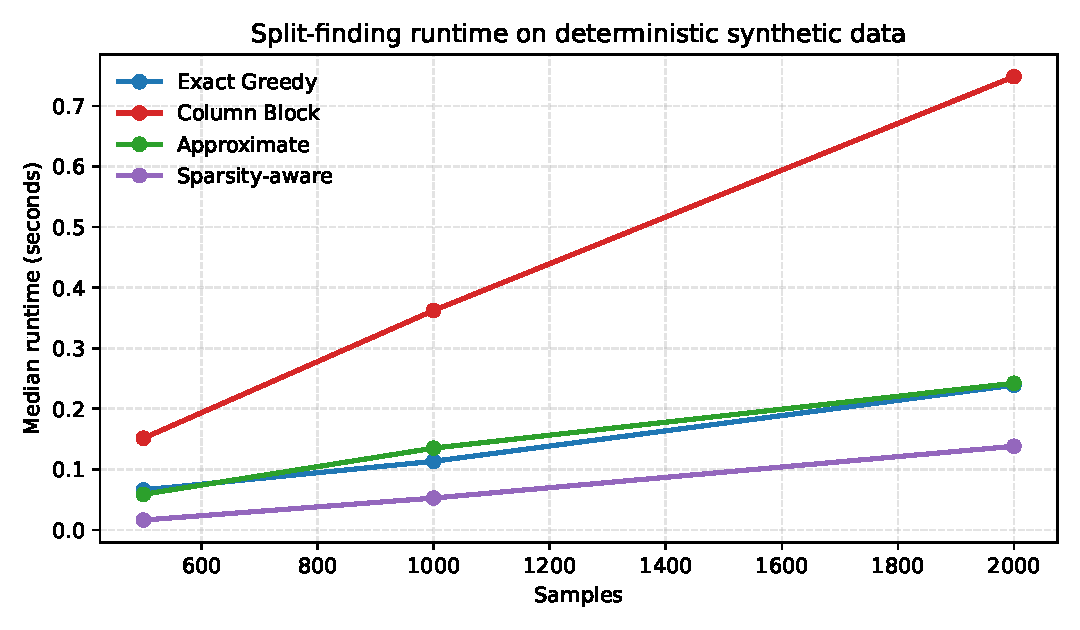
\includegraphics[width=0.82\textwidth]{images/runtime_comparison.pdf}
    \caption{So sánh runtime median giữa các thuật toán split finding}
    \label{fig:runtime_comparison}
\end{figure}

\subsection{Số candidate và gain}

Ngoài runtime, benchmark cũng ghi lại số candidate split được xét xấp xỉ và gain của split tốt nhất. Với $n=2000$ và $d=8$:

\begin{itemize}
    \item Exact Greedy và Column Block xét khoảng $15{,}992$ candidate trên dữ liệu dense.
    \item Approximate chỉ xét $160$ candidate do $\epsilon = 0.05$.
    \item Sparsity-aware xét khoảng $3{,}046$ candidate trên dữ liệu có $80\%$ missing.
\end{itemize}

Gain của Approximate thường nhỏ hơn Exact Greedy vì nhiều threshold bị bỏ qua. Đây là đánh đổi cốt lõi của approximate split finding: giảm chi phí bằng cách chấp nhận khả năng bỏ lỡ split tốt nhất.

\subsection{Nhận xét từ benchmark}

Kết quả cho thấy ba điểm chính.

Thứ nhất, Sparsity-aware Split Finding nhanh nhất trong benchmark này vì dữ liệu sparse chỉ có khoảng $20\%$ giá trị non-missing. Điều này phù hợp với phân tích độ phức tạp: khi số entry được scan giảm mạnh, thời gian chạy cũng giảm.

Thứ hai, Approximate Split Finding giảm rất mạnh số candidate. Tuy nhiên, bản Python hiện tại vẫn phải chia lại tập dữ liệu cho từng candidate, nên tốc độ chỉ nhỉnh hơn Exact Greedy trong một số cấu hình nhỏ. Trong cài đặt tối ưu hơn, các thống kê theo bucket có thể giúp tận dụng tốt hơn lợi thế $q \ll n$.

Thứ ba, Column Block trong benchmark này chậm hơn Exact Greedy. Nguyên nhân đến từ chi phí phụ của bản minh họa Python: lọc active row, cấp phát danh sách tạm và tạo thứ tự giảm dần khi xét default direction. Vì vậy, benchmark này không nên được dùng để kết luận rằng Column Block là chậm; nó chỉ cho thấy bản cài đặt hiện tại chưa tối ưu ở mức hệ thống.

\subsection{Liên hệ với phân tích độ phức tạp}

Thực nghiệm củng cố một thông điệp quan trọng: cùng một ý tưởng thuật toán có thể cho kết quả khác nhau tùy mức độ tối ưu của cài đặt.

Ở mức lý thuyết, Exact Greedy tốn chi phí vì xét gần như toàn bộ threshold, Approximate giảm số candidate, Sparsity-aware giảm số entry cần scan, và Column Block giảm việc sort lặp lại. Ở mức code Python minh họa, lợi ích này chỉ thể hiện rõ nhất với Sparsity-aware, trong khi Approximate và Column Block vẫn chịu overhead đáng kể.

Do đó, khi đọc benchmark, cần tách hai lớp kết luận:

\begin{itemize}
    \item \textbf{Kết luận thuật toán}: các kỹ thuật của XGBoost giảm chi phí bằng cách giảm sort, giảm candidate hoặc giảm entry scan.
    \item \textbf{Kết luận implementation}: bản Python trong repository minh họa đúng ý tưởng, nhưng chưa tối ưu như hệ thống XGBoost thật.
\end{itemize}
